\documentclass[a4paper]{article}

\usepackage[utf8]{inputenc}
\usepackage[T1]{fontenc}
\usepackage{textcomp}
\usepackage[english]{babel}
\usepackage{amsmath, amssymb}
\usepackage{physics}


% figure support
\usepackage{import}
\usepackage{xifthen}
\pdfminorversion=7
\usepackage{pdfpages}
\usepackage{transparent}
\newcommand{\incfig}[1]{%
	\def\svgwidth{\columnwidth}
	\import{./figures/}{#1.pdf_tex}
}

\pdfsuppresswarningpagegroup=1
\title{PH 550 - Soft Matter Physics}
\begin{document}
\section{Introduction}
AKA Soft Condensed Matter Physics (MC mai ghoom phir ke CMP pe aa gya).  Course content
\begin{enumerate}
	\item Intro to soft matter
	\item Viscoelasticity
	\item Colloids
	\item Polymers
	\item Surfactants
	\item Liquid Crystals
\end{enumerate}

Books
\begin{itemize}
	\item Soft Matter Physics (Richard Jones)
	\item Soft Matter Physics (Masao Doi)
	\item Introduction to the Theory of Soft Matter (Jonathan Selinger) [liquid crystals]
\end{itemize}

So, there's three adjectives in front of the word `Physics'.

\subsection{Matter}
Composed of atoms or molecules. Matter refers to collections of atoms
and molecules. Don't go about referring to a single atom as `matter'.

It is expected that when we say `matter', we have a very large ($\approx N_A$) number
of building components. 

So, how does  one go about dealing with such
systems? Statistical physics. Your Hamiltonian formalism and Newton's
equations will shit the bed.

Solid systems and gaseous systems are easy to deal with for Physicists,
because some really neat approximations can be made. In liquids, however
potential energy $\approx$ kinetic energy.

[Missed some part of the lecture]

An example of Helium's phase diagram was given. There is a critical
pressure below which it cannot exist in the liquid state. Point was
$P>0$ for the existence of liquid, or something like that. You need
pressure for  the existence of liquids.

You see, the world is not just made up of solid, liquid and gas only.
Like what the fuck even is the phase of toothpaste and shampoo??

\begin{figure}[h]
	\centering
	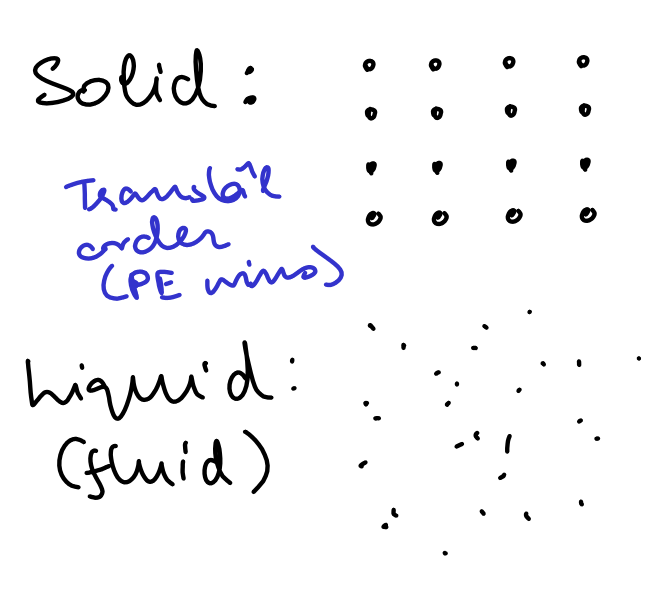
\includegraphics[width=0.8\textwidth]{figures/order.png}
	\caption{Fluids vs solids - order}
	\label{fig:figures-order-png}
\end{figure}

\begin{itemize}
	\item Solid
		\begin{itemize}
			\item Translational order
			\item translationally broken symmetry
			\item  broken rotational symmetry
		\end{itemize}
	\item Fluid
		\begin{itemize}
			\item Translationally disordered
			\item translationally symmetric
			\item rotational symmetries  preserved
		\end{itemize}
\end{itemize}

Deformations are not energetically favourable in solids and hence
any attempts to move  particles by shearing, compressing etc will
result in strong restoring forces.

Fluids on the other hand have 0 elastic moduli

Then  we have soft matter  systems, where the elastic moduli are
somewhere in between the above two  cases.

Systems like liquid crystals  are again quite unique because 
\begin{itemize}
	\item  Rotational order
	\item No translational order
\end{itemize}

BTW time scales matter. Phase diagrams don't  show time, only
thermodynamic parameters. But, we generally think of different phases
like solids, liquids etc in terms of their response funcions - their dynamics.
If something is hard, it's solid. If something flows, it's liquid.
Phase diagrams do not really capture the dynamics  properly.

\subsection{Grading}
\begin{itemize}
	\item Home assignments - 33\%
	\item Midsem - 33\%
	\item Endsem - 33\%
\end{itemize}

\section*{Intermolecular Forces}
Must be attractive at some ranges (else cannot have condensed phases), corresponding potential should achieve minima somewhere.
\begin{figure}[h]
	\centering
	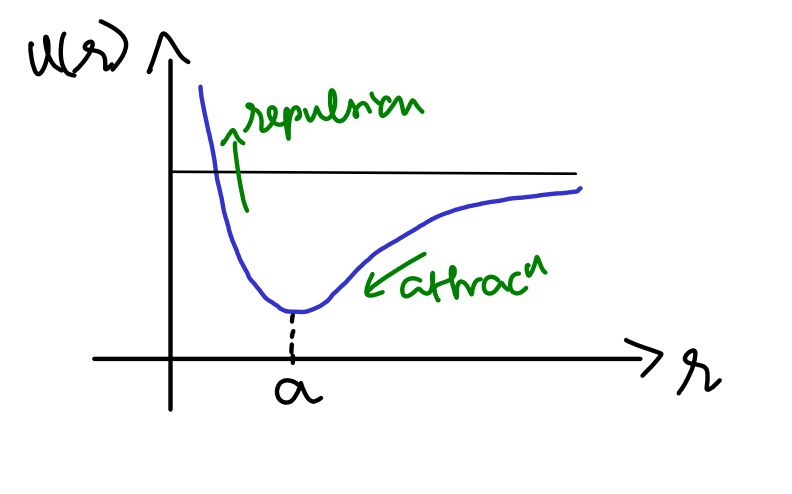
\includegraphics[width=0.8\textwidth]{figures/attr.png}
	\caption{Typical interatomic potentials in condensed matter systems}
	\label{fig:figures-attr-png}
\end{figure}

\begin{equation}
	\begin{split}
		&r\to \infty \implies -\frac{\dd U}{\dd r} = 0\\
		&r \ge a \implies -\frac{\dd U}{\dd r} \le  0\\
		&r < a \implies -\frac{\dd U}{\dd r} > 0
	\end{split}
\end{equation}

\subsection*{Metallic Bond}
A simple minded picture - positive cores form a lattice and negative
carriers dispersed throughout the material. Coulomb forces responsible
for holding the metallic bulk together. 

Typical strength $\approx 10^{-18}$ J $\approx 6 $ eV, around
300 Kelvin.

\subsection*{Ionic Bonds}
Similar bond energy as metallic bonds, bulk formed by interpenetrating
lattices of positive and negative charge cores.

\subsection*{Covalent Bonds}
Electron sharing and all that jazz. Typically weaker than ionic bonds

\subsection*{Van der Waals interactions}
Initiated by spontaneous polarization of a molecule, which then
polarizes nearby molecules and the overall medium can be modelled
using some empirical potentials that simulate this interaction.

This is typically the weakest interaction,  $k_BT \approx $ room temp. $U\sim \frac{1}{r^{6}}$
 
\subsection*{Hydrogen Bonds}
O, F, N et cetera participate in Hydrogen bonding. refer to CBSE book
nothing new here really.

\begin{figure}[h]
	\centering
	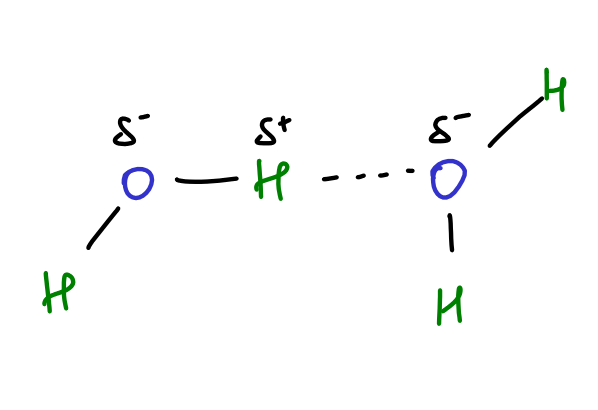
\includegraphics[width=0.8\textwidth]{figures/hydrogen.png}
	\caption{Hydrogen bonding in water}
	\label{fig:figures-hydrogen-png}
\end{figure}

This gives rise to non-trivial properties, like the density of ice
being lesser than the density of water. Bond strenth $\sim 20 - 100 k_B$

\section*{What is `soft' matter}
We generally think of colloids, liquid crystals etc. The basic
building units are mesoscopic in size (somewhere between micro and macro).

Where an atom is typically of the order of a few angstroms, soft matter
building blocks are somewhere from a few nanometers to microns.

Consider the act of compressing some bulk material. We define the
bulk modulus of the medium as 
\begin{equation}\label{bulk}
	\kappa = \frac{\Delta P}{\Delta V/V}
\end{equation}

\begin{figure}[h]
	\centering
	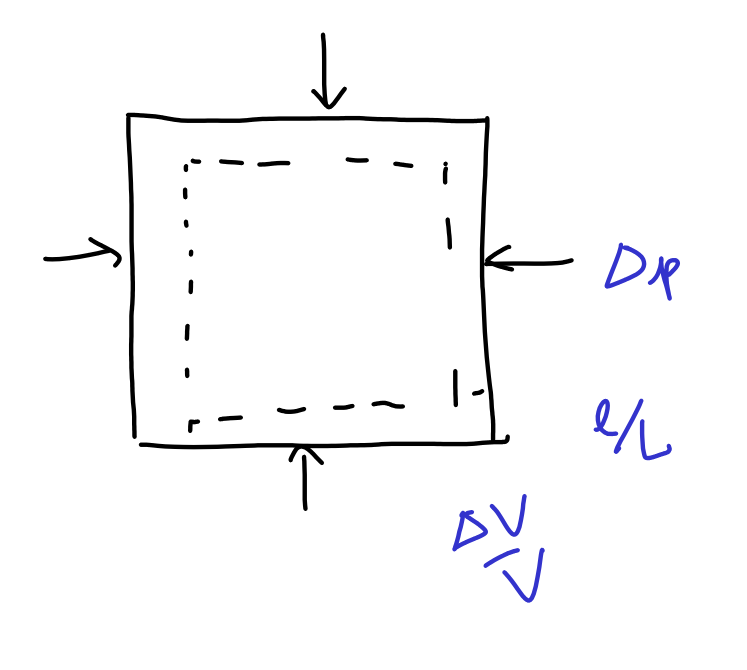
\includegraphics[width=0.8\textwidth]{figures/bulkmod.png}
	\caption{Doing a bulk compression}
	\label{fig:figures-bulkmod-png}
\end{figure}
Bulk moduli for condensed matter are very high, because the structure
of the bulk material is maintained by the interatomic forces, which
typically have a very narrow minimum range. Compressing those solids
requires one to reduce the average interatomic distances, thus increasing
thus making the restoring force highly repulsive.

Similarly, we could also shear a bulk material. Shear modulus
\begin{equation}
	G = \sigma \frac{L}{l}
\end{equation}
where $\sigma = F/A$ is the shear stress and $\gamma = l/L$ or $\Delta L / L$is the
sheer strain (see figure \ref{fig:sheer})

\begin{figure}[h]
	\centering
	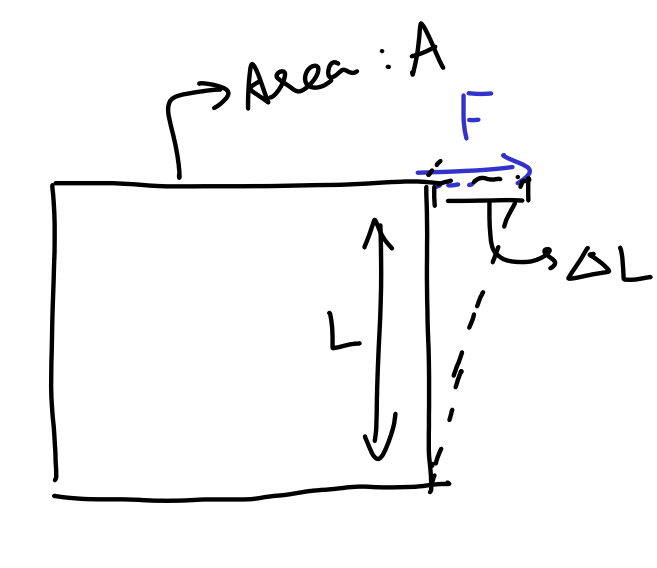
\includegraphics[width=0.8\textwidth]{figures/sheer.png}
	\caption{Sheer modulus}
	\label{fig:sheer}
\end{figure}

Why do soft materials have low $G$?
% TODO: Complete this

Consider the toy model in figure \ref{fig:spring-png} made using springs.

\begin{figure}[h]
	\centering
	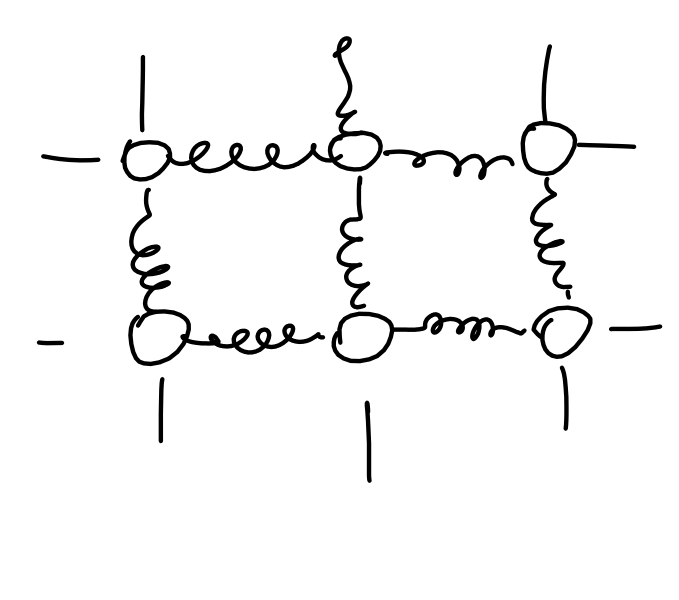
\includegraphics[width=0.8\textwidth]{figures/spring.png}
	\caption{}
	\label{fig:spring-png}
\end{figure}
If we try to deform it, then we have
\begin{equation}
	\begin{split}
		&F = k(r - a)\\
		\text{Stress,}\quad&\sigma = \frac{F}{A} = \frac{d(r-a)}{a^2}\\
			\text{Strain,}\quad &\gamma = \frac{r-a}{a}\\
			\text{Young's modulus,}\quad &Y = \frac{\sigma}{\gamma} = \frac{k(r-a)}{a^2(r -a)}\vdot a = \frac{k}{a}
	\end{split}
\end{equation}

During deformation that doesn't straight up destroy the whole bulk
material, we are essentially moving in a small window around the
potential minimum (see fig \ref{fig:figures-attr-png}), we can Taylor
expand the potential to get some harmonic dynamics.

\begin{equation}
	U(r) = U(a) - \frac{1}{2!}\dv[2]{U}{r} \left( r -a \right) ^2
\end{equation}

% TODO: complete the equations

\subsection*{Some important properties of soft matter systems}
%%% TODO
\begin{enumerate}
	\item Disordered matter: energy scales $\approx k_B T$, e.g. granular matter
	\item Nonlinear matter
	\item Far from equilibrium matter
	\item Thermal and entropic matter: 
	\item Observable matter: 
\end{enumerate}

Summary: Young's modulus $E \approx \frac{\epsilon}{a^3}$, where
$\epsilon \to  \text{typical bond strength}, a \to  \text{bond length}$ %%%% TODO: verify what exactly  $a$ is

\section*{Viscous, elastic, and viscoelastic behaviour}
\begin{itemize}
	\item Solid: It resists shear stress and undergoes shear strain without yielding, i.e. original shape et cetera is restored.
	\item Liquid: Cannot susteain shear stress and yields (i.e. it flows)
\end{itemize}

Based on this we can define a Hookean solid
\begin{equation}
	\sigma = \frac{F}{A} \quad \text{Shear stress} 
\end{equation}
\begin{equation}
	\gamma = \frac{\Delta x}{y} \quad \text{Shear strain}
\end{equation}
\begin{equation}
	\text{Shear modulus,} \quad G = \frac{\sigma}{\gamma}
\end{equation}
is the modulus associated with all Hookean solids.

Similarly we can define a Newtonian liquid
\begin{equation}
	\sigma = \frac{F}{A}
\end{equation}
\begin{equation}
	\text{Shear strain rate,} \quad \dot{\gamma} = \frac{\Delta x}{y\vdot t} = \frac{v}{y}
\end{equation}
\begin{equation}
	\frac{\sigma}{\dot{\gamma}} = \eta \quad \text{(Shear viscosity)}
\end{equation}

Why Newtonian? Assumed that $\eta$ is constant, i.e. not a function of 
$\dot{\gamma}$

\begin{figure}[h]
	\centering
	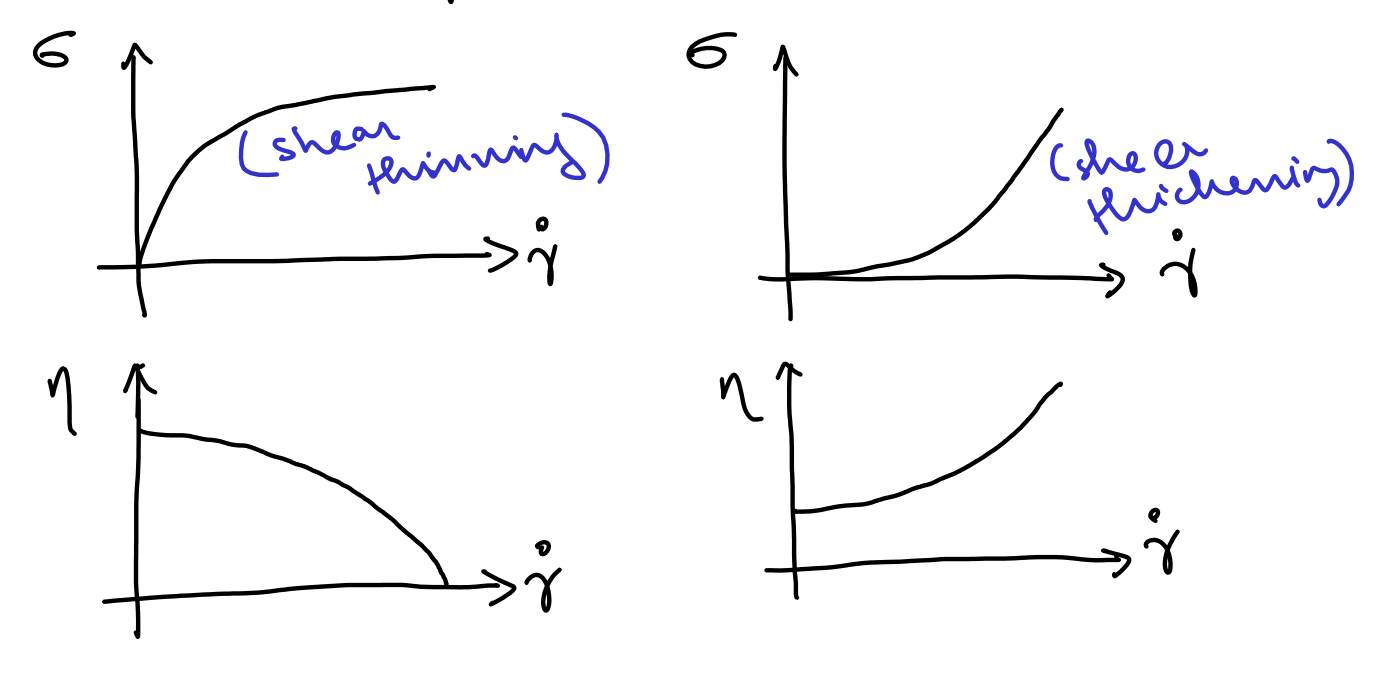
\includegraphics[width=0.8\textwidth]{figures/nonnewtonian.png}
	\caption{Sheer thickening vs sheer thinning non-Newtonian fluids, driving the system increases and decreased viscosity respectively}
	\label{fig:figures-nonnewtonian-png}
\end{figure}

\begin{itemize}
	\item Newtonian $\to $ Water
	\item Shear thinning $\to $ Shampoo, Ketchup
	\item Shear thickening $\to $ those corn starch solutions that people keep forwarding on WhatsApp.
\end{itemize}

Similarly, we can also have non-Hookean solids. For solids, we have
$G = \sigma/\gamma$. We know that end of the day, metals also yield,
which is why bridges, for example are not meant to last forever.
\begin{figure}[h]
	\centering
	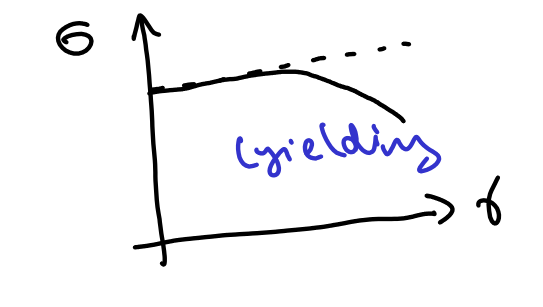
\includegraphics[width=0.8\textwidth]{figures/nonhooke.png}
	\caption{Yielding in solids - nothing is ideal, of course}
	\label{fig:figures-nonhooke-png}
\end{figure}

\subsection*{How do viscoelastic materials respond to stress?}
Consider the the rig that is used to apply stress, measure strain
and all that. The material being tested could be solid or liquid (or
something really in between).
\begin{figure}[h]
	\centering
	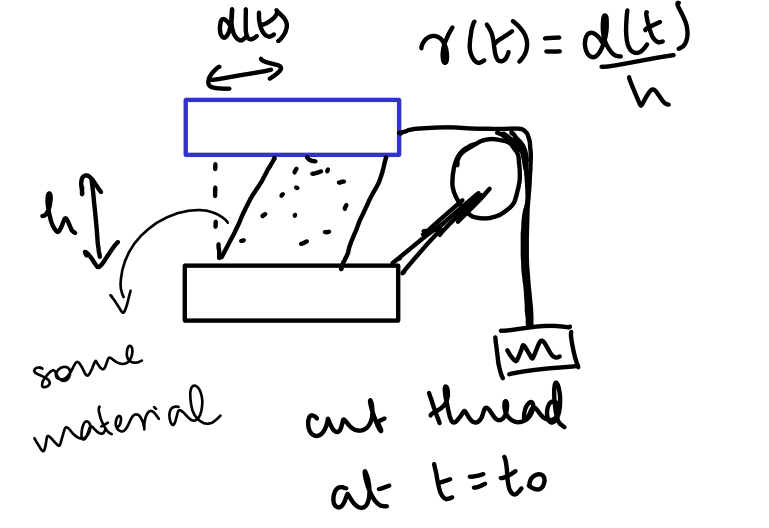
\includegraphics[width=0.8\textwidth]{figures/rig.png}
	\caption{A rig used to apply stress and measure response of the material}
	\label{fig:figures-rig-png}
\end{figure}

\begin{figure}[h]
	\centering
	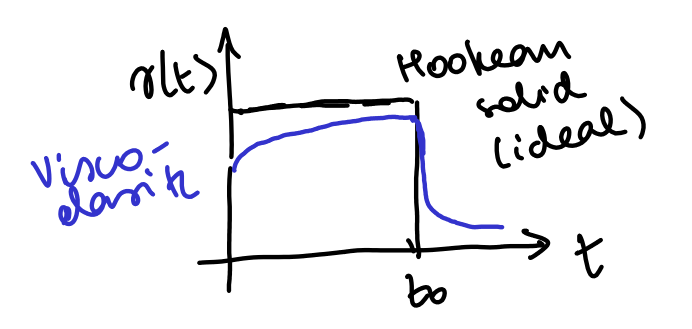
\includegraphics[width=0.8\textwidth]{figures/viscoelasticresponse.png}
	\caption{Response of ideal (Hookean) and real (non-Hookean) solid}
	\label{fig:figures-nonhooke-png}
\end{figure}

Similarly we could compare liquids
\begin{figure}[h]
	\centering
	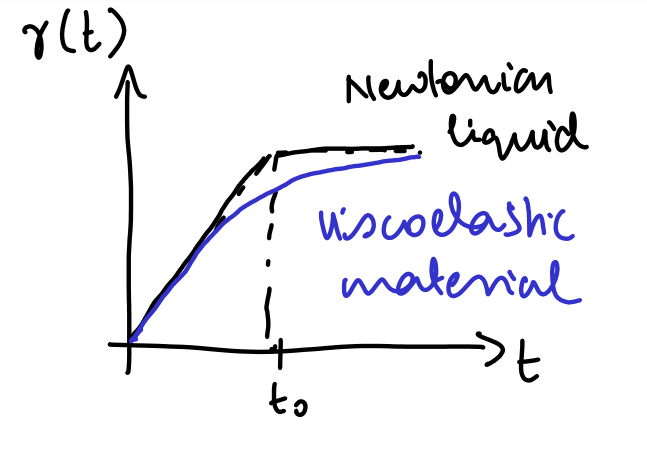
\includegraphics[width=0.8\textwidth]{figures/l.png}
	\caption{Ideal (Newtonian) vs viscoelastic liquid responses}
	\label{fig:l-png}
\end{figure}	

\begin{figure}[h]
	\centering
	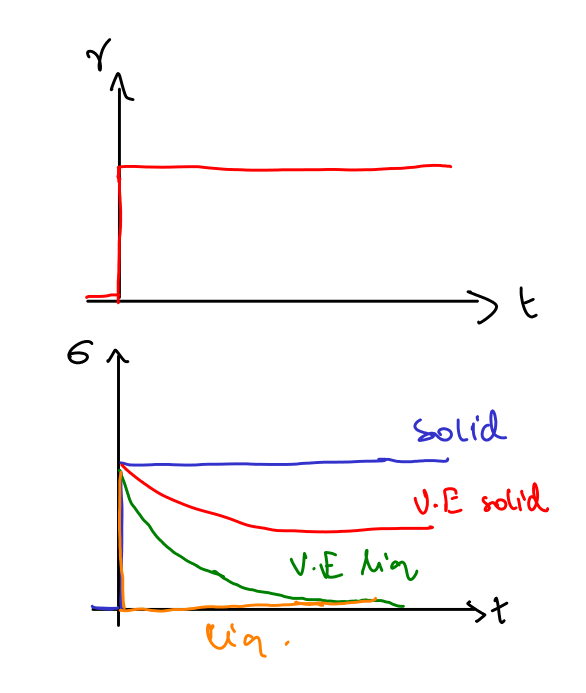
\includegraphics[width=0.8\textwidth]{figures/responsesummary.png}
	\caption{Comparison between the different classes of condensed matter systems to sheer stress}
	\label{fig:figures-summary}
\end{figure}
% 
\subsection*{Concept of relaxation time}
\begin{equation}
	\begin{split}
		&\sigma = G \gamma \to  \text{solid}\\
		&\sigma = \eta \dot{\gamma} \to \text{liquid}
	\end{split}
\end{equation}

The relaxation time $\tau$ is the time below which system has an
elastic response.

\textbf{Deborah number:} It is a way of distringuishing between
solids and liquids based on ratio of relaxation time and observation
time.

``Even the mountains flow before God"

God can see mountains flow. Nothing religious going on here.

\begin{equation}
	\text{Deborah number,}\quad D_e = \frac{\text{Relaxation time}}{\text{Observation time}}
\end{equation}

\begin{equation}
	\begin{split}
		&D_e \to  \text{high} \to Solid\\
		&D_e \to  \text{low} \to  liquid	
	\end{split}
\end{equation}

Everything flows on a long enough time scale. (See the article on Deborah number that
appeared in Physics Today in 1964). To have a small $D_e$ you can
either have a small relaxation time, or a very large ovservation time
for an otherwise long relaxation time.

%%%% TODO: lots of stuff LMAO
%%%% The following notes are from lecture 5
\section*{Linear Viscoelasticity}
We want to calculate the response of a soft matter system to some
arbitrary strain $\gamma(t)$. 
\begin{equation}
	\sigma(t) = \int_{-\infty}^tG(t-t')\dot{\gamma}(t')\dd t'
\end{equation}

Consider an oscillatory stress \[
	\gamma(t) = \gamma_0 \cos\omega t
.\] 

The response of a linear medium is a superposition of an elastic term.
Our response function will be of the form
\begin{equation}
	G^{*}(\omega) = G'(\omega) + iG''(\omega)
\end{equation}
The first term is the elastic response (storage) and the second one
is the viscous response (loss modulus). Note that we are assuming
that the system has a single relaxation time.

and a viscour term
\begin{equation}
	%%%% TODO:
	G'(\omega) = G_{e} + \frac{G(\omega\tau)}{LOL}
\end{equation}

So far we are ignoring molecular structure of the soft material. Once
we start doing system-specific studies, e.g. polymers, surfactants et
cetera, then we'll look at more accurate descriptions. Nevertheless,
these approximations give, in many cases, some meaningful insight.

\subsubsection*{Mechanical Elements}
Simple models of linear media are typically constructed using spring-dashpot 
models. The spring (Young's modulus $E$) emulates the elastic part of the response while the
dashpot (or damper, viscosity $\eta_E$) emulates the viscous response.

So, we have
\begin{equation}
	\begin{split}
		\sigma = E\gamma\\
		\sigma= \eta_E \dot{\gamma}
	\end{split}
\end{equation}

\begin{equation}
	\eta_E = \tau E, %%% TODO: there was another response function/expression to distinguish between something idk
\end{equation}
where $\tau$ is the relaxation time of the material.

For a spring-dashpot series model, we have
\begin{equation}
	\sigma = \sigma_s = \sigma_d
\end{equation}

The difference lies in the strain experienced by the two elements
\begin{equation}
	\begin{split}
		&\gamma = \gamma_s + \gamma_d\\
		\implies &\dot{\gamma} = \dot{\gamma}_s + \dot\gamma_d\\
		\implies & \sigma_s = E\gamma_s\quad \text{and}\\
			 &\sigma_d = \eta_E \dot\gamma_d
	\end{split}
\end{equation}

These are the equations for extension, but the same can be done for
shear stress.

Creep: Apply tensile stress $\sigma_{E,0}$ which is held
		constant at later time (i.e. step input)
\begin{equation}
	\dv{\sigma}{t} = 0 \implies \dv{\sigma_s}{t} = 0
\end{equation}
\begin{equation}
	\implies \dv{\sigma_{E,0}}{t} = %%% TODO
\end{equation}
\begin{equation}
	\begin{split}
		\int_0^t \dd \gamma &= \int_0^t \frac{\sigma_{E,0}}{\eta_E}\dd t \\
		\implies \gamma(t) - \gamma(0) &= \sigma_{E,0}\frac{t}{\eta_E} \\
		\implies \frac{\gamma(t)}{\sigma_{E,0}} &= \frac{\gamma(0)}{\sigma_{E,0}} + \frac{t}{\eta_E} 
	\end{split}
\end{equation}

Tensile compliance is defined as the inverse of the Young's modulus.
%%% TODO: I have the attention span of a labrador

Something-something dynamic experiment.

\begin{equation}
	\sigma_E(t) = \sigma^{*}_{E,0}e^{i\omega t}
\end{equation}
We have the equation for the Maxwell element
\begin{equation}
	\dv{\gamma}{t} = \frac{1}{E} \dv{\sigma_E}{t} = \frac{\sigma_E}{\eta_E}
\end{equation}
\end{document}
